\chapter{Arhitectura soluţiei}
\label{chapter:arhitecture}

\section{Prezentare generală}
Sistemul de achiziţie, procesare şi distribuţie a datelor a fost conceput ca o platformă de dezvoltare rapidă, bazat pe modele. Utilizatorul poate să îşi concentreze resursele asupra soluţiei finale, abstractizând detaliile implementării prin folosirea unor metode de programare vizuală, cu blocuri refolosibile în mai multe aplicaţii diferite. 
Aplicaţia a fost construită pe baza unei arhitecturi modulare; modulele fiind cât mai puţin interconectate, permiţând modificări rapide şi testarea modulelor individual. Urmărind aceasta gândire modulare s-au identificat 4 componente esenţiale: 
\begin{itemize}
	\item \textbf{Baza de date} Asigură stocarea datelor şi a entităţilor existente;
	\item \textbf{Interfaţa web pentru management} O interfaţă uşor de utilizat care permite  utilizatorului să manipuleze canale, diagrame, blocuri de procesare, dar şi alţi utilizatori
	\item \textbf{API-ul pentru date} Un API specializat pentru achiziţia de  date şi să permită informarea altor dispozitive cu privire la apariţia unor date noi.
	\item \textbf{Elemente de procesare} Asigură procesarea datelor, atât în cadrul blocurilor de procesare, cât şi în cadrul diagramelor funcţionale.
\end{itemize}
\begin{figure}
	\centering
	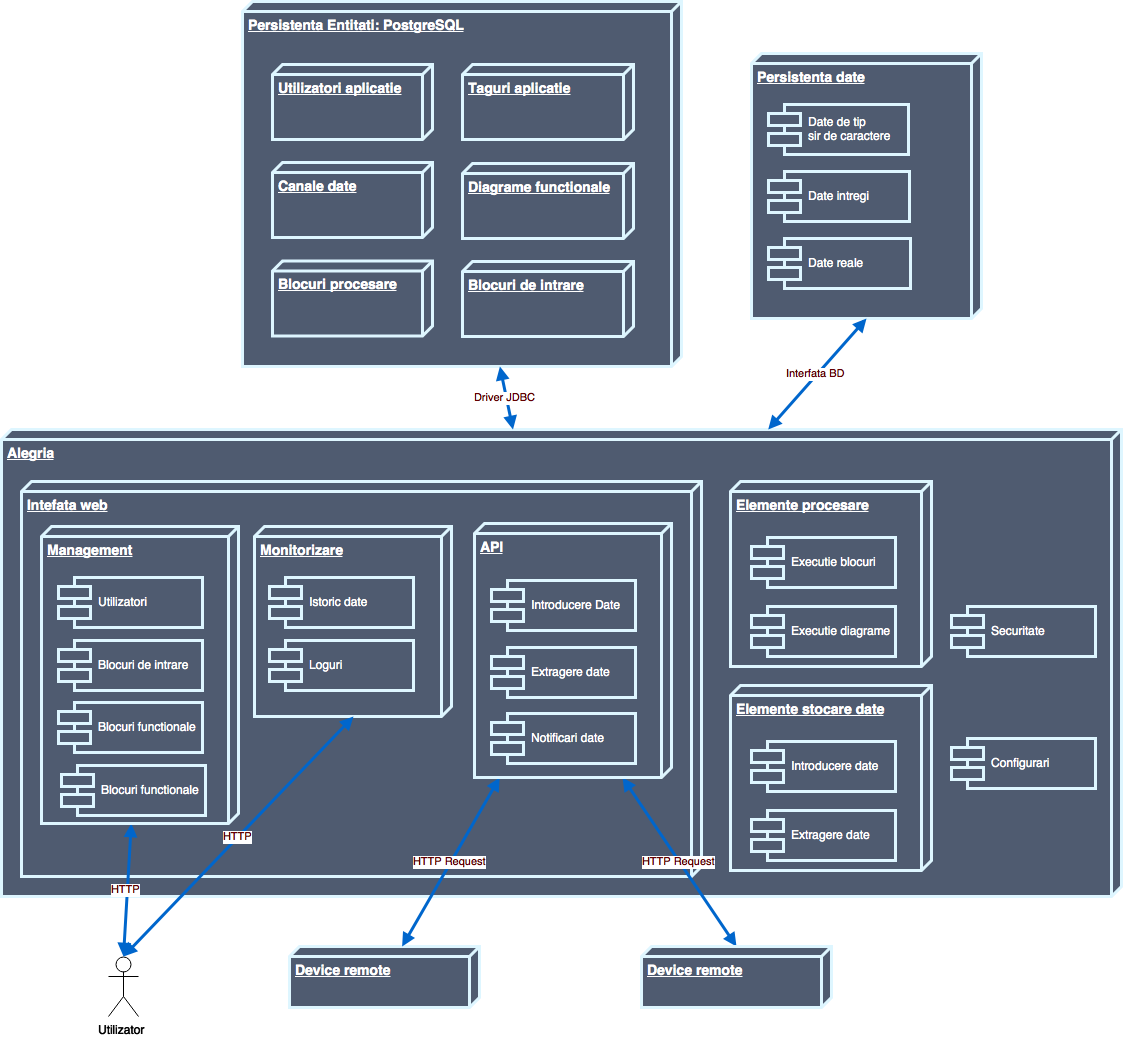
\includegraphics[width=1.3\textwidth, center]{arhitecturaGenerala}
	\caption{Arhitectura generala a aplicaţiei}
	\label{fig:arhitecture}
\end{figure}

În vederea implementării sistemului s-au identificat următoarele elemente componente esenţiale, componente ce reprezintă elementele constructive a sistemului. Acestea au reprezentare atât în baza de date, ca entităţi, cât şi în aplicaţia Java, ca clase. Identificarea acestor elemente s-a făcut pe baza analizei cazurilor de utilizare ale produsului în care s-au investigat metodele prin actorii interacţionează cu sistemul.
\begin{itemize}
	\label{list:entities}
	\item \textbf{Canalul de date} Reprezintă elementul de bază a sistemului ce asigură recepţia, persistenţa şi emiterea de date.  La crearea canalului, datele dintr-un canal, trebuie să respecte un format prestabilit. Pentru transformarea datelor în formatul stabilit se poate introduce un bloc de pre-procesarea care transformă datele din formatul brut în formatul standard;
	\item \textbf{Blocul de intrare} Elementul ce mapează un element din lumea real în interiorul platformei. Blocurile de intrare permit gruparea mai multor canale de date într-o structura unică;
	\item \textbf{Blocul de procesare} Elementul dinamic al aplicaţiei ce aplică transformări asupra datelor. Un bloc de procesare primeşte ca intrări mai multe canale de date şi are la ieşire un alt canal de date. Utilizatorul poate folosi blocuri standard, existente în sistem, sau poate implementa blocuri noi direct în interfaţa programului;
	\item \textbf{Diagrama funcţie bloc(FBD)} Foloseşte blocuri de intrare, canale de date şi blocuri de procesare pentru a descrie o funcţie complexă între 0-n intrări şi o ieşire. Aceste diagrame folosesc datele - aflate pe canalele de date - ce sunt trimise către blocurile de procesare şi la final se obţine un singur rezultat care este salvat pe un canal de date.
\end{itemize}

\subsection{Baza de date}

Fiind vorba despre o aplicaţie puternic bazata pe date, aceasta are nevoie de un nivel de persistenţă de înaltă performaţă. 
Urmărind arhitectura propusă din \cref{fig:arhitecture}, putem identifica două cazuri de utilizare pentru baza de date: 
\begin{itemize}
	\item Stocarea modelului entităţilor: fiecare entitate descrisă în lista de mai sus trebuie stocată în baza de date, într-o structură relaţională. Entităţile sunt puternic interconectate şi de aceea este recomandată o baza de date relaţională, de tip SQL. 
	Din punct de vedere a dimensiunii setului de date, chiar şi în aplicaţiile de mare complexitate, este vorba despre câteva milioane de înregistrări. Factorul care face acest număr să crească este conectarea a tot mai mult dispozitive, ce duce la din ce în ce mai multe canale de date. Astfel, stocarea entităţilor nu va aduce probleme de performaţă. 
	\item Stocarea datelor: în baza de date vor fi stocate atât datele primite pe fiecare canal asociat unui bloc de intrare, cât şi datele procesate de diagrame. Aceste date au un puternic caracter istoric, reprezentând o serie de timp în care se reţine  valoarea fiecărui punct de date la un anumit moment. Problema stocării acestor date este una mai complicată datorită necesităţii unei puternice scalari a bazei de date. Această problemă reprezintă un caz de utilizare pentru o baza de date NoSQL sau chiar o baza de date specializata în stocarea seriilor de timp \autocite{openTSDB}.  
\end{itemize}

\subsection{Aplicaţia Java}
Legătura dintre baza de date şi utilizatorii finali se face prin intermediul unei aplicaţii Java complexe, care este obiectul acestui proiect. Aplicaţia conţine toată logica platformei, de la operaţii asupra entităţilor din baza de date, la adăugarea,  extragerea şi procesarea datelor. 
Separarea modulelor s-a făcut pe baza scopului acestora astfel:
\begin{itemize}
	\item \textbf{Administrare}: pentru administrarea entităţilor din baza de date. Aceste module permit atât operaţii de căutare şi afişare, cât şi de creere, editare şi ştergere a utilizatorilor, a blocurilor de intrare şi funcţionale, şi a diagramelor. Fiecare dispune de o interfaţă HTML5;
	\item \textbf{Monitorizare}: permit monitorizarea execuţiei aplicaţiei de la vizualizat loguri pentru a diagnostica probleme până la realizarea de grafice a datelor pe anumite canale. Tot aici este disponibilă şi funcţia de a exporta date în formate uzuale (CSV, fişiere Microsoft Excel, etc);
	\item \textbf{API}: aplicaţia dispune şi de un API pentru a fi folosit programatic de către alte aplicaţii externe. Acesta este format din două componente: servicii pentru administrarea entităţilor şi servicii pentru adăugarea şi extragerea datelor;
	\item \textbf{Elemente de procesare}: sunt împărţite în două subcategorii: cele pentru procesarea blocurilor de intrare şi de procesare, şi cele pentru procesarea diagramelor;
	\item \textbf{Elemente stocare date}: permit interfaţarea cu sursele de date. Prin intermediul unei interfaţe abstractă, acestea asigură servicii de introducere şi extragere a datelor care nu ţin cont de modul în care baza de date este implementată;
	\item \textbf{Alte module}: asigură, printre altele securitatea aplicaţiei.
\end{itemize}

\section{Entităţi}
\subsection{Punctul de date}

Punctul de date reprezintă elementul constructiv al sistemul reprezentând obiectul procesării, stocării şi distribuţiei. 
Sistemul accepta intern date în formatele: 
\begin{wrapfigure}{r}{0.38\textwidth}
	\centering
	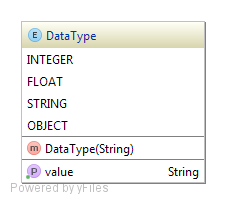
\includegraphics[width=0.38\textwidth]{dataType}
	\caption{Tipurile de date acceptate în sistem}
\end{wrapfigure}
\begin{itemize}
	\item \textbf{Întreg}: numere în intervalul $(-2^{63}, 2^{63} -1)$, fără virgulă; foloseşte \textit{Long} pentru reprezentare internă;
	\item \textbf{Real}: numere cu virgulă, având dubla precizie, reprezentate pe 64-bit conform standardului \autocite{4610935} IEEE 754;  foloseşte \textit{Double} pentru reprezentare internă;
	\item \textbf{Sir de caractere}: Un şir de caractere fără lungime limită ce trebuie formatat conform \autocite{rfc4627}. 
	\item \textbf{Obiect}: Un obiect Java serializat în text. Intern, asemănător cu tipul de date String. 
\end{itemize}

\begin{figure}[h]
	\centering
	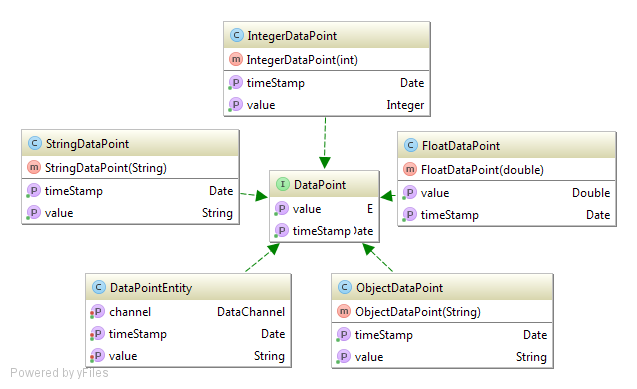
\includegraphics[width=1.1\textwidth, center]{dataPoint}
	\caption{Clasele care implementează interfaţa DataPoint}
\end{figure}

\subsection{Canalul de date}

Canalul de date este entitatea care asigura "curgerea" datelor prin sistem. Orice punct de date din sistem aparţine unui canal, acest lucru fiind realizat drept constrângere atât la nivelul aplicaţiei, cât şi la nivelul bazei de date.
\begin{figure}[h]
	\centering
	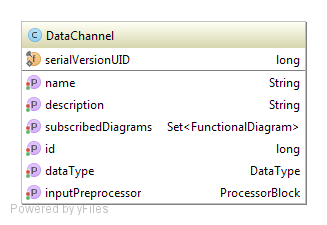
\includegraphics[width=0.55\textwidth]{dataChannel}
	\caption{Clasa DataChannel}
\end{figure}

Canalul de date este şi mijlocul prin care utilizatorul interacţionează cu punctele de date. Când un dispozitiv adaugă date noi în sistem, acestea sunt ataşate unui canal  care poate fi folosit ca una dintre intrările unei diagrame de blocuri funcţionale. De asemenea, datele procesate de o diagramă sunt ataşate unui canal, permiţând apoi accesul pentru extragerea de datelor deja existente şi pentru a primi notificări de fiecare dată când pe un canal apar informaţii noi.

În plus, un canal de date poate avea şi un bloc de preprocesare ataşat. Acesta este executat de fiecare data când date noi încearcă să fie introduse în canal, permiţând validarea şi transformarea datelor brute în date ce respectă tipul de date al canalului.  
\subsection{Blocul de intrare}
Blocurile de intrare modelează elemente reale în Alegria, grupând mai multe canale de date şi expunându-le pentru a permite introducerea datelor din exterior. Acestea descriu modul în care datele sunt legate de un element real. 

Spre exemplu, o sursa inteligentă si conectată de alimentare neîntreruptibilă din \cref{fig:ups} poate fi privită ca un bloc de intrare, unde fiecare senzor este reprezentat de un canal de date. Dispozitivul inteligent devine astfel conectat la platforma şi acesta poate sa trimită date către aceasta. Pentru ca datele pot sa aibă perioade de eşantionare diferite, dispozitivul trimite date de la unul sau mai mulţi senzori odată, fiecare canal de date fiind tratat individual.

Un alt mod în care blocurile de intrare pot fi privite este ca obiecte, sau "Things" în cadrul Internetului Tuturor Lucrurilor (IoT). Astfel, putem privi blocurile de intrare ca dispozitive ce monitorizează bătăile inimii sau activitatea celebrară, ca automobile cu reţele complexe de senzori, sau chiar aplicaţii business ce generează date în timp real. Prin acest mijloc, dispozitive inteligente se pot conecta în platforma, fie trimiţând direct date, fie prin intermediul unui agent care se afla pe dispozitiv, agent ce funcţionează ca un gateway, implementând protocoale proprietare de comunicaţie.

\begin{figure}[H]
	\centering
	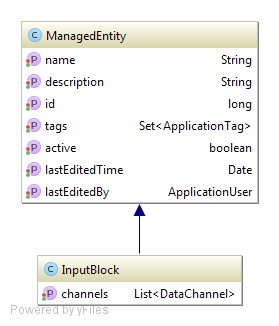
\includegraphics[width=0.55\textwidth]{inputBlock}
	\caption{Clasa \textbf{InputBlock}}
\end{figure}
\begin{figure}[H]
	\centering
	\includegraphics[width=\textwidth]{UPS}
	\caption{Modelarea unui UPS inteligent în Alegria}
	\label{fig:ups}
\end{figure}

\subsection{Blocul de procesare}

Blocurile de procesare realizează operaţiile transformare a datelor. Din punct de vedere funcţional, acestea au la intrare ultimele date introduse de pe mai multe canale şi returnează un singur punct de date, comportându-se ca un element de tip "back-box"\autocite{functionBlocks}. Pentru implementare, utilizatorul foloseşte limbaje dinamice moderne, ca JavaScript sau Ruby, scriind cod direct în interfaţa web. Acest cod este rulat de către server. 
Conceptul de blocuri de procesare reprezinta o implementare a blocurilor de operaţii definite în standardul  IEC61131-3 \autocite[Apendix C]{IEC61131-3} .

Blocuri pre-implementate, existente în orice instantă a platformei, permit rezolvarea de probleme complexe cu cunoştinţe minime de programare.
Un alt aspect important al blocurilor de procesare, este faptul ca sunt independente de sursa de date, ele oferind doar mijloace de prelucrare a unor date abstracte. Aceasta abstractizare permite refolosirea lor în mai multe proiecte. Spre exemplu, un bloc care face media tuturor intrărilor nu tine cont de originea datelor. 

Blocurile \textbf{nu au memorie statica}. Ele pot folosi informaţii exterioare, cum ar fi timpul curent al zilei, sau alte informaţii din sistem, sau pot chiar accesa servicii web, însa ele nu au stare interioară. Astfel, se poate considera ca blocurile reprezintă un element combinaţional, şi nu unul secvenţial.
\begin{figure}[H]
	\centering
	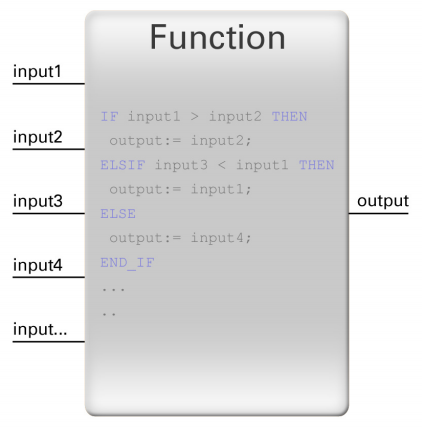
\includegraphics[width=0.55\textwidth]{exempluBlock}
	\caption{Exemplu bloc de procesare}
\end{figure}

\begin{figure}[H]
	\centering
	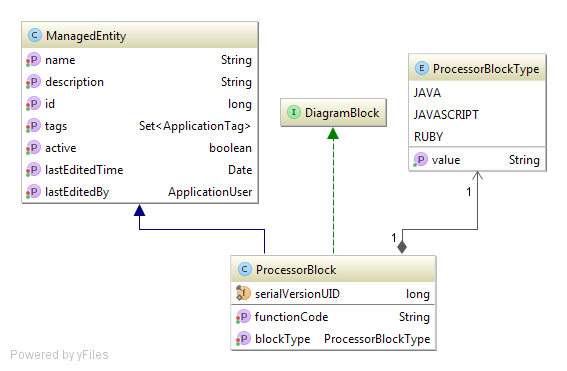
\includegraphics[width=\textwidth]{processorBlock}
	\caption{Clasa \textbf{ProcessorBlock}}
\end{figure}

\subsection{Diagrama funcţie bloc(FBD)}

Diagramele funcţie bloc reprezintă o implementare a unuia din cele patru limbare de programare pentru automate programabile, specificate de standardul IEC 61131-3:2013 \autocite[128-140]{IEC61131-3}. FBD-ul este un limbaj de control al procesului, iar, în mod normal, toate blocurile de procesare dintr-o diagrama sunt executate.
In cel mai simplu caz de utilizare, un FBD realizează următoarele operaţii:
\begin{itemize}
	\item Acceptă date de intrare de la unul sau mai multe canale;
	\item Realizează o operaţie de transformare asupra acelor date folosind un bloc de procesare;
	\item Salvează rezultatul pe un canal de ieşire.
\end{itemize}
Legăturile dintre blocuri sunt unidirecţionale. Un bloc de procesare poate trimite rezultatul său la unul sau mai multe blocuri, iar o intrare poate fi conectată la o singura ieşire. Transmiterea de date se face fără întârzieri. Diagramele sunt executate în ordinea definita de ordonarea topologica a nodurilor din graful ce defineşte diagrama \autocite[20-50]{IEC61499}. 
\begin{figure}[H]
	\centering
	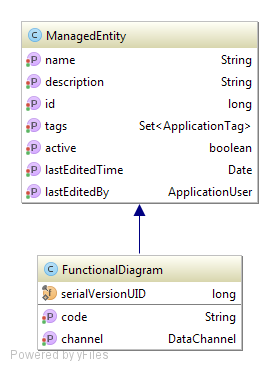
\includegraphics[width=0.5\textwidth]{functionalDiagram}
	\caption{Clasa \textbf{FunctionalDiagram}}
\end{figure}

\begin{figure}[H]
	\centering
	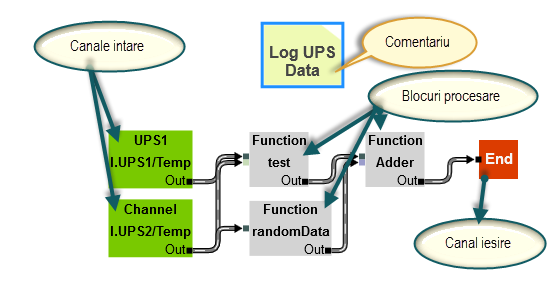
\includegraphics[width=0.95\textwidth]{exempluDiagrama}
	\caption{Exemplu diagrama funcţională}
	\label{fig:exempluDiagrama}
\end{figure}

\section{Primirea datelor}
Primirea datelor se face prin intermediul unei interfeţe de transfer a stării (REST). Mai multe formate acceptate pentru integrarea mai uşoară cu sisteme deja existente. Astfel, au fost implementate mai multe procesoare care primesc date atât într-un format nou, caracteristic aplicaţiei, cât şi în formate standard din industrie.
In această versiune, modalităţi de trimitere a datelor au fost implementate:
\begin{itemize}
	\item Trimitere către un singur canal, un singur punct odată: pe baza serviciului\\ \textit{/api/put/{inputId}/{channelId}/{data}}. Acest serviciu adaugă un singur punct în baza de date, la momentul curent. Folosit pentru sisteme care trimit date rar, şi nu trebuie sa se tina cont de data locala de pe device-ul care a trimis punctul de date.
	\item În formatul standard folosit de openTDSB, cu următoarele modificări care păstrează totuşi compatibilitatea: metricile reprezinta numele canalului, iar tag-urile sunt opţionale. Se acceptat atât formatul în care într-o cerere se afla un singur punct, cat şi formatul cu o lista de puncte. Canalele dintr-o cerere multidimensionala nu trebuie sa facă parte din acelaşi bloc de intrare. Acest mod de introducere a datelor este sugerat pentru sistemele care folosesc mai multe canale de date şi care trimit seturi de date mai mari printr-o singura cerere. Spre exemplu, un dispozitiv poate trimite date de pe mai multi senzori, şi poate stoca local mai multe măsurători pe acelaşi senzor pentru a trimite toate datele odată.
\end{itemize}
Odată primite, noile puncte de date trec prin procesul descris în \cref{fig:intrareDate}:
\begin{enumerate}
	\item Se interoghează baza de date pentru detalii privind canalul ce tocmai a primit date.
	\item Dacă un preprocesor exista pe canalul specificat, atunci el este încărcat.
	\item Se executa preprocesorul cu punctul de date primit.
	\item Se salvează rezultatul în baza de date.
	\item Asincron, se lansează toate diagramele care trebuie sa se execute atunci când se primesc date noi pe acest canal.
	\item Asincron, se informează ascultătorii ca canalul a primit date noi.
\end{enumerate}
\begin{landscape}
	\begin{figure}
		\centering
		\includegraphics[width=1.7\textwidth]{introducereDate}
		\caption{Diagrama de secvenţe pentru introducerea de noi date şi execuţia diagramelor}
		\label{fig:intrareDate}
	\end{figure}
\end{landscape}
